\documentclass[twoside]{book}

% Packages required by doxygen
\usepackage{fixltx2e}
\usepackage{calc}
\usepackage{doxygen}
\usepackage[export]{adjustbox} % also loads graphicx
\usepackage{graphicx}
\usepackage[utf8]{inputenc}
\usepackage{makeidx}
\usepackage{multicol}
\usepackage{multirow}
\PassOptionsToPackage{warn}{textcomp}
\usepackage{textcomp}
\usepackage[nointegrals]{wasysym}
\usepackage[table]{xcolor}

% Font selection
\usepackage[T1]{fontenc}
\usepackage[scaled=.90]{helvet}
\usepackage{courier}
\usepackage{amssymb}
\usepackage{sectsty}
\renewcommand{\familydefault}{\sfdefault}
\allsectionsfont{%
  \fontseries{bc}\selectfont%
  \color{darkgray}%
}
\renewcommand{\DoxyLabelFont}{%
  \fontseries{bc}\selectfont%
  \color{darkgray}%
}
\newcommand{\+}{\discretionary{\mbox{\scriptsize$\hookleftarrow$}}{}{}}

% Page & text layout
\usepackage{geometry}
\geometry{%
  a4paper,%
  top=2.5cm,%
  bottom=2.5cm,%
  left=2.5cm,%
  right=2.5cm%
}
\tolerance=750
\hfuzz=15pt
\hbadness=750
\setlength{\emergencystretch}{15pt}
\setlength{\parindent}{0cm}
\setlength{\parskip}{3ex plus 2ex minus 2ex}
\makeatletter
\renewcommand{\paragraph}{%
  \@startsection{paragraph}{4}{0ex}{-1.0ex}{1.0ex}{%
    \normalfont\normalsize\bfseries\SS@parafont%
  }%
}
\renewcommand{\subparagraph}{%
  \@startsection{subparagraph}{5}{0ex}{-1.0ex}{1.0ex}{%
    \normalfont\normalsize\bfseries\SS@subparafont%
  }%
}
\makeatother

% Headers & footers
\usepackage{fancyhdr}
\pagestyle{fancyplain}
\fancyhead[LE]{\fancyplain{}{\bfseries\thepage}}
\fancyhead[CE]{\fancyplain{}{}}
\fancyhead[RE]{\fancyplain{}{\bfseries\leftmark}}
\fancyhead[LO]{\fancyplain{}{\bfseries\rightmark}}
\fancyhead[CO]{\fancyplain{}{}}
\fancyhead[RO]{\fancyplain{}{\bfseries\thepage}}
\fancyfoot[LE]{\fancyplain{}{}}
\fancyfoot[CE]{\fancyplain{}{}}
\fancyfoot[RE]{\fancyplain{}{\bfseries\scriptsize Generated by Doxygen }}
\fancyfoot[LO]{\fancyplain{}{\bfseries\scriptsize Generated by Doxygen }}
\fancyfoot[CO]{\fancyplain{}{}}
\fancyfoot[RO]{\fancyplain{}{}}
\renewcommand{\footrulewidth}{0.4pt}
\renewcommand{\chaptermark}[1]{%
  \markboth{#1}{}%
}
\renewcommand{\sectionmark}[1]{%
  \markright{\thesection\ #1}%
}

% Indices & bibliography
\usepackage{natbib}
\usepackage[titles]{tocloft}
\setcounter{tocdepth}{3}
\setcounter{secnumdepth}{5}
\makeindex

% Hyperlinks (required, but should be loaded last)
\usepackage{ifpdf}
\ifpdf
  \usepackage[pdftex,pagebackref=true]{hyperref}
\else
  \usepackage[ps2pdf,pagebackref=true]{hyperref}
\fi
\hypersetup{%
  colorlinks=true,%
  linkcolor=blue,%
  citecolor=blue,%
  unicode%
}

% Custom commands
\newcommand{\clearemptydoublepage}{%
  \newpage{\pagestyle{empty}\cleardoublepage}%
}

\usepackage{caption}
\captionsetup{labelsep=space,justification=centering,font={bf},singlelinecheck=off,skip=4pt,position=top}

%===== C O N T E N T S =====

\begin{document}

% Titlepage & ToC
\hypersetup{pageanchor=false,
             bookmarksnumbered=true,
             pdfencoding=unicode
            }
\pagenumbering{alph}
\begin{titlepage}
\vspace*{7cm}
\begin{center}%
{\Large Projeto 3 -\/ Parte 2 }\\
\vspace*{1cm}
{\large Generated by Doxygen 1.8.14}\\
\end{center}
\end{titlepage}
\clearemptydoublepage
\pagenumbering{roman}
\tableofcontents
\clearemptydoublepage
\pagenumbering{arabic}
\hypersetup{pageanchor=true}

%--- Begin generated contents ---
\chapter{Hierarchical Index}
\section{Class Hierarchy}
This inheritance list is sorted roughly, but not completely, alphabetically\+:\begin{DoxyCompactList}
\item Q\+Main\+Window\begin{DoxyCompactList}
\item \contentsline{section}{Main\+Window}{\pageref{class_main_window}}{}
\end{DoxyCompactList}
\end{DoxyCompactList}

\chapter{Class Index}
\section{Class List}
Here are the classes, structs, unions and interfaces with brief descriptions\+:\begin{DoxyCompactList}
\item\contentsline{section}{\mbox{\hyperlink{class_main_window}{Main\+Window}} }{\pageref{class_main_window}}{}
\end{DoxyCompactList}

\chapter{Class Documentation}
\hypertarget{class_main_window}{}\section{Main\+Window Class Reference}
\label{class_main_window}\index{Main\+Window@{Main\+Window}}


Inheritance diagram for Main\+Window\+:

\hypertarget{class_plotter}{}\section{Plotter Class Reference}
\label{class_plotter}\index{Plotter@{Plotter}}
Inheritance diagram for Plotter\+:\begin{figure}[H]
\begin{center}
\leavevmode
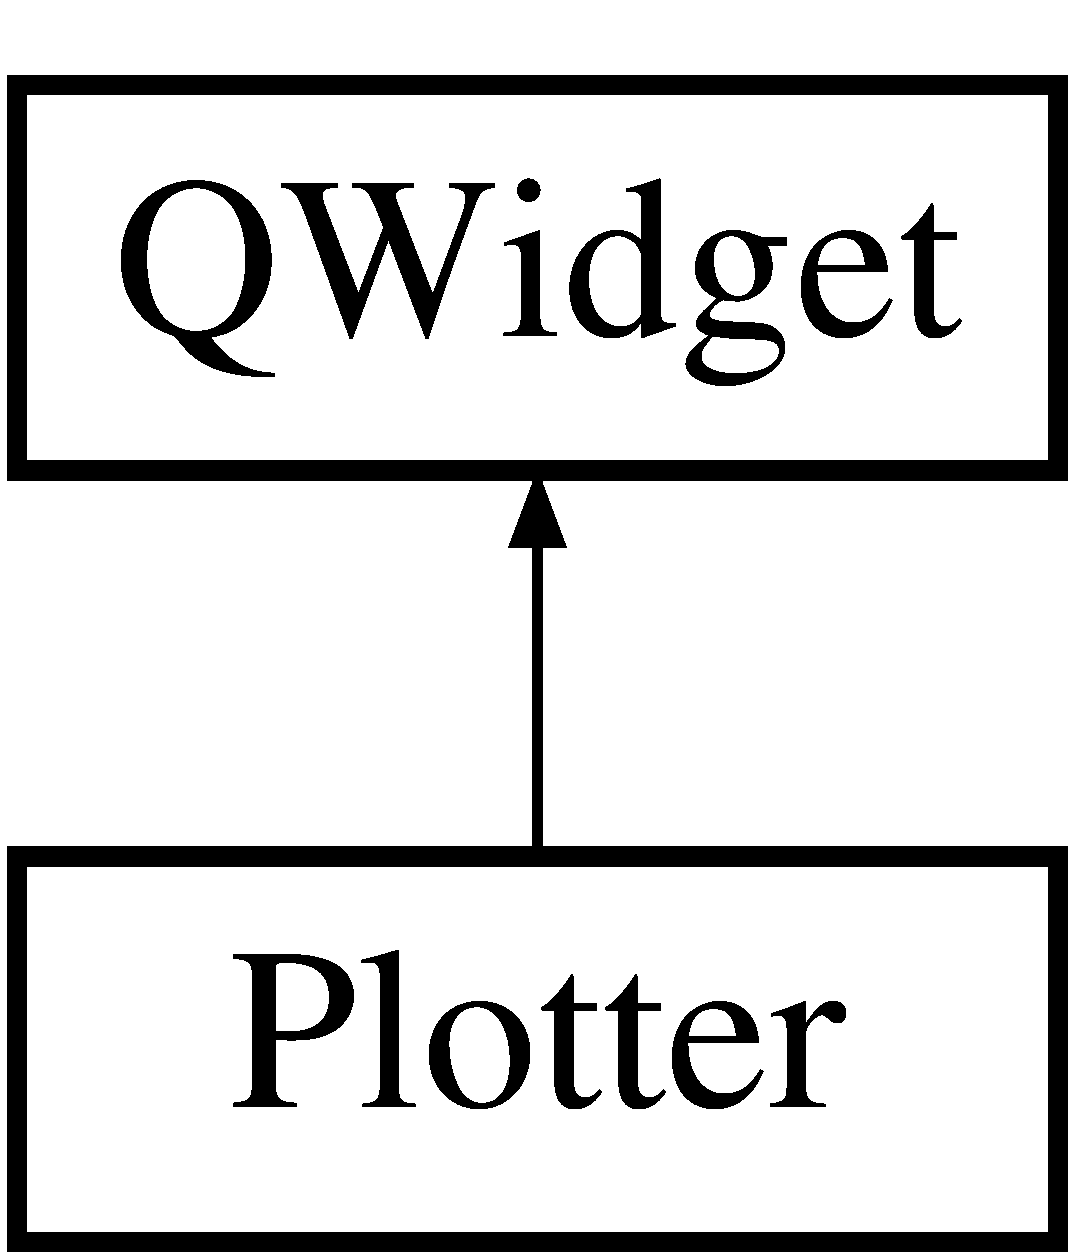
\includegraphics[height=2.000000cm]{class_plotter}
\end{center}
\end{figure}
\subsection*{Public Member Functions}
\begin{DoxyCompactItemize}
\item 
\mbox{\Hypertarget{class_plotter_a1807627530de30ae58dff3c42a823497}\label{class_plotter_a1807627530de30ae58dff3c42a823497}} 
{\bfseries Plotter} (Q\+Widget $\ast$parent=nullptr)
\item 
void \mbox{\hyperlink{class_plotter_a06477bf987646f000a8982db1352a11d}{paint\+Event}} (Q\+Paint\+Event $\ast$event)
\begin{DoxyCompactList}\small\item\em \mbox{\hyperlink{class_plotter_a06477bf987646f000a8982db1352a11d}{Plotter\+::paint\+Event}} Realiza o desenho da tela. \end{DoxyCompactList}\item 
void \mbox{\hyperlink{class_plotter_a29034483f5519c5bf9dac3ac849e0466}{plot\+Grafico}} (vector$<$ qint64 $>$ \&t, vector$<$ int $>$ \&v)
\begin{DoxyCompactList}\small\item\em \mbox{\hyperlink{class_plotter_a29034483f5519c5bf9dac3ac849e0466}{Plotter\+::plot\+Grafico}} Realiza a plotagem do gráfico. \end{DoxyCompactList}\end{DoxyCompactItemize}


\subsection{Member Function Documentation}
\mbox{\Hypertarget{class_plotter_a06477bf987646f000a8982db1352a11d}\label{class_plotter_a06477bf987646f000a8982db1352a11d}} 
\index{Plotter@{Plotter}!paint\+Event@{paint\+Event}}
\index{paint\+Event@{paint\+Event}!Plotter@{Plotter}}
\subsubsection{\texorpdfstring{paint\+Event()}{paintEvent()}}
{\footnotesize\ttfamily void Plotter\+::paint\+Event (\begin{DoxyParamCaption}\item[{Q\+Paint\+Event $\ast$}]{event }\end{DoxyParamCaption})}



\mbox{\hyperlink{class_plotter_a06477bf987646f000a8982db1352a11d}{Plotter\+::paint\+Event}} Realiza o desenho da tela. 


\begin{DoxyParams}{Parameters}
{\em event} & \\
\hline
\end{DoxyParams}
painter

brush

pen\mbox{\Hypertarget{class_plotter_a29034483f5519c5bf9dac3ac849e0466}\label{class_plotter_a29034483f5519c5bf9dac3ac849e0466}} 
\index{Plotter@{Plotter}!plot\+Grafico@{plot\+Grafico}}
\index{plot\+Grafico@{plot\+Grafico}!Plotter@{Plotter}}
\subsubsection{\texorpdfstring{plot\+Grafico()}{plotGrafico()}}
{\footnotesize\ttfamily void Plotter\+::plot\+Grafico (\begin{DoxyParamCaption}\item[{vector$<$ qint64 $>$ \&}]{t,  }\item[{vector$<$ int $>$ \&}]{v }\end{DoxyParamCaption})}



\mbox{\hyperlink{class_plotter_a29034483f5519c5bf9dac3ac849e0466}{Plotter\+::plot\+Grafico}} Realiza a plotagem do gráfico. 


\begin{DoxyParams}{Parameters}
{\em t} & \\
\hline
{\em v} & \\
\hline
\end{DoxyParams}


The documentation for this class was generated from the following files\+:\begin{DoxyCompactItemize}
\item 
plotter.\+h\item 
plotter.\+cpp\end{DoxyCompactItemize}

%--- End generated contents ---

% Index
\backmatter
\newpage
\phantomsection
\clearemptydoublepage
\addcontentsline{toc}{chapter}{Index}
\printindex

\end{document}
